%!TEX encoding = UTF-8 Unicode
%!TEX root = ../compendium.tex

\Lab{\LabWeekELEVEN}

\begin{Goals}
\item Kunna använda inbyggda sorteringsfunktioner \code{sortBy} och \code{sortWith}.
\item Kunna implementera insättningssortering till ny sekvens.
\item Känna till hur strängar ordnas.
\item Kunna använda registrering (frekvensräkning). 
\item Kunna använda matriser med strängar.
\end{Goals}

\begin{Preparations}
\item \StudyTheory{10}
\item \DoExercise{\ExeWeekELEVEN}{11} Träna speciellt på insättningssortering till ny sekvens.
\item \ReadTheLab 
\item Studera den givna koden i workspace för labben \code{survey2} \textbf{Obs. 2:an!} 
\item Fyll i denna enkät: \url{https://goo.gl/forms/hC6JK2UQXVpbGECc2}  \\
I enkäten ska du för olika flervalsalternativlistor besvara frågan: \\ \textit{Vilket är ditt favoritalternativ?}
\end{Preparations}


\subsection{Bakgrund}

I den här veckans laboration ska du utveckla ett program som analyserar svar på enkäter med flervalsfrågor. Indata utgörs av text i form av \textbf{kolumnseparerade värden}, där varje persons svar finns på en egen rad och varje svarsrad innehåller svarsalternativ. 
Exempelindata finns i filen \code{favorit.csv} i mappen resources:
\lstinputlisting[basicstyle=\ttfamily\fontsize{10}{12}\selectfont]{../workspace/w10_survey/src/main/resources/favorit.csv}
Kolumnerna är separerade med en \textbf{kolumnseparator} som t.ex. kan vara \code{"\t"} eller \code{","}. Första raden i textfilen anger kolumnernas namn.


\subsection{Obligatoriska uppgifter}

\Task Implementera case-klassen \code{Table} för sortering, filtrering, registrering av strängmatriser med titelrad, enligt nedan specifikationen.

\begin{ScalaSpec}{Table}
case class Table(matrix: Vector[Vector[String]],
                 headings: Vector[String],
                 separator: String) {

  /** Returns the number of (rows, columns) of the matrix data. */
  val dim: (Int, Int) = ???

  /** Returns the values from a specified column. */
  def col(c: Int): Vector[String] = ???

  /** Returns the matrix in string format using separator between columns*/
  override lazy val toString: String = ???

  /** A new Table with rows sorted on column c (implemented using sortBy). */
  def sort(c: Int): Table = ???

  /** A new Table with rows sorted on column c (implemented from scratch). */
  def mySort(c: Int): Table = ???

  /**
   * A new Table filtered so that column c only contains the wanted values.
   */
  def filter(c: Int, wanted: Vector[String]): Table = ???

  /**
   * Returns the distinct values for the given column coupled with the number
   * of occurrences for that value. The pairs are sorted descending on the
   * number of occurrences. The first element is the column header together
   * with the total number of occurrences for all values.
   */
  def register(c: Int): Vector[(String, Int)] = ???
}
\end{ScalaSpec}


Till din hjälp finns följande kod given i workspace: 
\begin{itemize}
\item \code{Main} sätter igång användarinteraktionen och hanterar undantag.

\item \code{Command} sköter läs-evaluera-skriv-loopen i programmet.

\item \code{Chart} ritar diagram i \code{SimpleWindow}.

\item Kompanjonsobjektet \code{Table} har den färdig fabriksmetoden \code{fromFile} för inläsning av kolumnseparerad data och konstruktion av \code{Table}-instanser, och kan även spara tabeller i filer med den färdiga metoden \code{save}.
\end{itemize}

\noindent Du hittar koden här:
\href{https://github.com/lunduniversity/introprog/tree/master/workspace/w10_survey2/src/main}{https://github.com/lunduniversity/introprog/tree/master/\\workspace/w10\_survey2/src/main}




\Task Testa systematiskt alla kommandon med olika parametrar och kontrollera så att alla delar av \code{Table} fungerar korrekt. Nedan exempelkörning visar hur testandet kan gå till.

\begin{REPLnonum}
*** Welcome to stats for table data ***

Current dir: /home/bjornr/lthgitlab/pgk/solution-workspace/w10_survey_v2/bin/
Type 'help' for list of commands.
> help
Commands: help
             Prints this list of commands.
          load <location>
             Loads a table from <location> using , as separator
          load <location> <separator>
             Loads a table from <location> using <separator>
          save <filepath>
             Saves the table to <filepath>
          sep <separator>
             Changes the separator of the table
          filter <column> <values: a b c>
             Filters the table so <column> only contains <values>
          sort <column>
             Sorts the table on <column>
          mysort <column>
             Sorts the table on <column> using my own sort implementation
          print
             Prints the table to the console
          printchart <column>
             Prints a barchart of <column> to the console
          pie <column>
             Draws a pie chart of current table in a SimpleWindow
          bar <column>
             Draws a bar chart of current table in a SimpleWindow
          quit
             Terminates the program
> load favorit.csv
Loading favorit.csv with separator ',' to table ...

Done. Size: 17x7.

> print
Program,Indent,UI,Lang,OS,Browser,DE
D,Spaces,Terminal,C,BSD,Firefox,Emacs
C,Spaces,Terminal,Javascript,Windows 7,Chrome,Notepad++
D,Spaces,GUI,Java,macOS,Safari,Gedit
I,Tabs,Terminal,PHP,Windows 10,Edge,Notepad++
C,Spaces,GUI,Java,Windows 8,Firefox,Eclipse
D,Spaces,Terminal,Java,Windows 8,Edge,Eclipse
F,Spaces,Terminal,C,Linux,Chrome,Emacs
D,Spaces,GUI,C,Linux,Firefox,Vim
Nano,Tabs,Terminal,Javascript,macOS,Safari,Vim
C,Tabs,Terminal,C#,Windows 10,Edge,Visual Studio
D,Tabs,GUI,Javascript,macOS,Chrome,Emacs
D,Spaces,GUI,Python,Windows 7,Chrome,Notepad++
E,Spaces,Terminal,Java,Linux,Chromium,Eclipse
I,Tabs,Terminal,Python,Windows 10,Chrome,Notepad++
K,Tabs,GUI,C#,Windows 7,Firefox,Visual Studio
F,Spaces,Terminal,C,Linux,Firefox,Vim
D,Tabs,GUI,C,Linux,Chrome,Gedit
> filter 0 D
> print
Program,Indent,UI,Lang,OS,Browser,DE
D,Spaces,Terminal,C,BSD,Firefox,Emacs
D,Spaces,GUI,Java,macOS,Safari,Gedit
D,Spaces,Terminal,Java,Windows 8,Edge,Eclipse
D,Spaces,GUI,C,Linux,Firefox,Vim
D,Tabs,GUI,Javascript,macOS,Chrome,Emacs
D,Spaces,GUI,Python,Windows 7,Chrome,Notepad++
D,Tabs,GUI,C,Linux,Chrome,Gedit
> sep ;
> print
Program;Indent;UI;Lang;OS;Browser;DE
D;Spaces;Terminal;C;BSD;Firefox;Emacs
D;Spaces;GUI;Java;macOS;Safari;Gedit
D;Spaces;Terminal;Java;Windows 8;Edge;Eclipse
D;Spaces;GUI;C;Linux;Firefox;Vim
D;Tabs;GUI;Javascript;macOS;Chrome;Emacs
D;Spaces;GUI;Python;Windows 7;Chrome;Notepad++
D;Tabs;GUI;C;Linux;Chrome;Gedit
> sort 1
> print
Program;Indent;UI;Lang;OS;Browser;DE
D;Spaces;Terminal;C;BSD;Firefox;Emacs
D;Spaces;GUI;Java;macOS;Safari;Gedit
D;Spaces;Terminal;Java;Windows 8;Edge;Eclipse
D;Spaces;GUI;C;Linux;Firefox;Vim
D;Spaces;GUI;Python;Windows 7;Chrome;Notepad++
D;Tabs;GUI;Javascript;macOS;Chrome;Emacs
D;Tabs;GUI;C;Linux;Chrome;Gedit
> mysort 2
> print
Program;Indent;UI;Lang;OS;Browser;DE
D;Spaces;GUI;Java;macOS;Safari;Gedit
D;Spaces;GUI;C;Linux;Firefox;Vim
D;Spaces;GUI;Python;Windows 7;Chrome;Notepad++
D;Tabs;GUI;Javascript;macOS;Chrome;Emacs
D;Tabs;GUI;C;Linux;Chrome;Gedit
D;Spaces;Terminal;C;BSD;Firefox;Emacs
D;Spaces;Terminal;Java;Windows 8;Edge;Eclipse
\end{REPLnonum}

\Task Testa att programmet fungerar tillsammans med länken till enkätsvaren: \url{https://goo.gl/qPcuAO}

\clearpage

\subsection{Frivillig extrauppgift}

I den frivilliga extrauppgiften ska du implementera metoden \code{bar} i singelobjektet \code{Chart} som kan rita ut stapeldiagram enligt figuren nedan. Du har nytta av att studera koden i den befintliga metoden \code{pie}.
\begin{REPLnonum}
*** Welcome to stats for table data ***

Current dir: /home/bjornr/lthgitlab/pgk/solution-workspace/w10_survey_v2/bin/
Type 'help' for list of commands.
> load favorit.csv
Loading favorit.csv 
  with separator ',' to table ...

Done. Size: 17x7.

> pie 0
> bar 0
\end{REPLnonum}

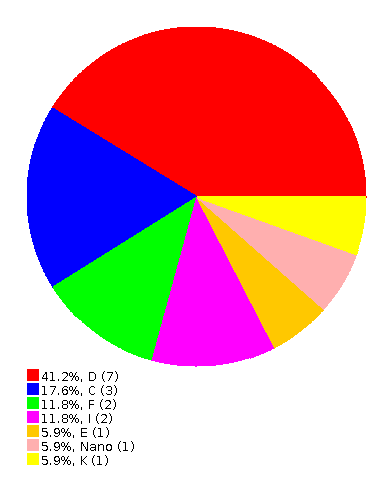
\includegraphics[width=0.5\textwidth]{../img/survey/pie.png}

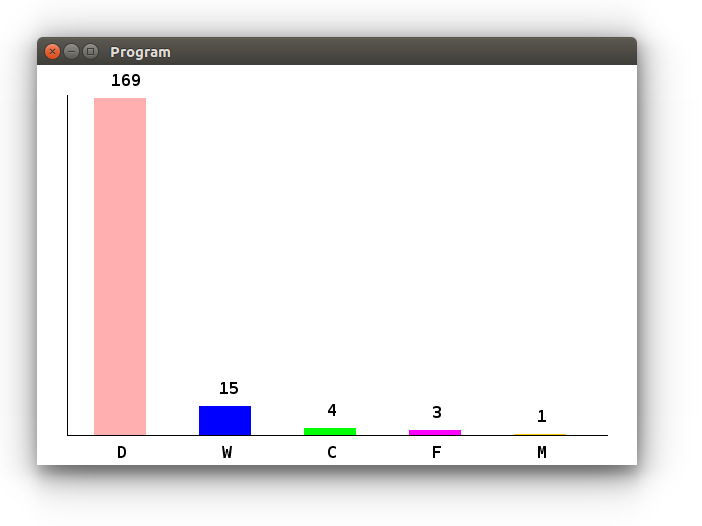
\includegraphics[width=0.7\textwidth]{../img/survey/bar.png}

